\section{Background and Motivation}
\label{sect:background}

\subsection{Definition of AI Agents}
\label{sect:llm_agent_definition}

AI agents are inference-time frameworks that extend the capabilities of LLMs by enabling multi-step reasoning, adaptive decision-making, and interaction with the external environment. Unlike conventional LLM applications that produce a single output from a static prompt, AI agents operate through iterative internal reasoning and external actions at inference time. At each iteration, the agent may generate an intermediate reasoning result, call an external tool (e.g., search engine, calculator, or code interpreter), and incorporate the output into its subsequent decisions. This process allows the agent to retrieve missing information and refine its strategy \emph{dynamically} in response to evolving task demands. While this adaptivity enhances the ability to handle complex and open-ended problems, it also leads to variability in the LLM calls, tool usage patterns, and overall computational cost.

\subsection{Core Components and Workflows of AI Agents}
\label{sect:llm_agent_components}

\begin{figure}[t!] \centering
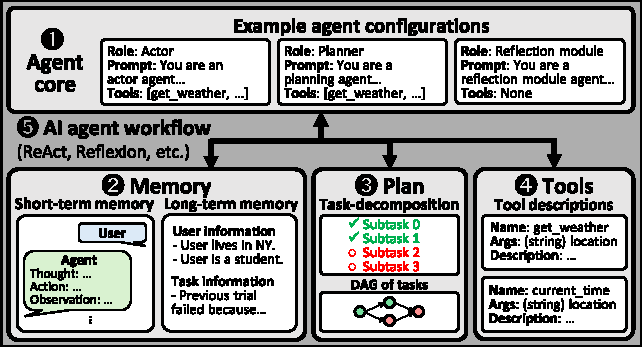
\includegraphics[width=0.48\textwidth]{./fig/agent_overview}\\
\vspace{-0.4em}    
\caption{\small Overview of AI agent structure.
}
\label{fig:agent_overview}
\vspace{-0.6em}    
\end{figure}

As illustrated in \fig{fig:agent_overview}, AI agents generally consist of four core components (\emph{agent core, memory, plan}, and \emph{tools}), and \emph{AI agent workflows} interconnect these core components through iterative interactions. These workflows orchestrate how the components dynamically collaborate, enabling the agent’s adaptive behaviors.

The \circlednum{1}~\emph{agent core} is the central component responsible for \emph{advanced reasoning}, powered by one or more LLMs configured in specific ``roles''. These roles typically include an \emph{actor}, which determines the agent’s next action; a \emph{planner}, which decomposes high-level goals into subtasks; and a \emph{reflection module}, which evaluates prior reasoning steps and tool interaction trajectories to guide future decisions.

This core reasoning capability of the AI agent is further supported by \emph{memory}, \emph{plan}, and \emph{tools}. \circlednum{2} \emph{Memory} plays a critical role in enabling the agent to maintain continuity across reasoning steps by storing short-term interaction traces as well as long-term knowledge, including user preferences or experience from past interactions. 
\circlednum{3} \emph{Plan} organizes the agent’s objective into a sequence of subtasks or a directed acyclic graph (DAG) of interdependent actions. By maintaining an explicit plan, the agent can prioritize actions, track progress, and make forward-looking decisions that align with the overall task structure.
\circlednum{4} \emph{Tools} extend the agent’s capabilities beyond text generation by enabling interaction with external environments. At each step, the agent analyzes its current context, generates a structured command specifying the desired tool and input, executes the tool call, and incorporates the resulting output into its context. This output is then used to guide the next stage of reasoning.

Finally, \circlednum{5}~\emph{AI agent workflow} defines how an agent leverages interactions among the four core components iteratively to carry out reasoning and coordinate actions. AI agents implement their own distinct workflows, reflecting different coordination patterns among components. These workflows can be broadly decomposed into two phases: (1) \emph{LLM inference phase}, where the agent performs internal reasoning tasks such as action generation, planning, or reflection; and (2) \emph{tool use phase}, where the agent interacts with external environments using tools. These two phases alternate iteratively, forming the backbone of AI agentic systems.

\subsection{Test-Time Scaling in AI Agents}

Test-time scaling refers to methods that improve the reasoning performance of pretrained LLMs at inference time by increasing the amount of computation used for inference without modifying model parameters~\cite{cot,tot,self_cot,least_cot,snell2024scalingllmtesttimecompute}. Representative techniques include Chain-of-Thought~\cite{cot}, which guides the model to produce intermediate reasoning steps through carefully crafted prompts, and Tree-of-Thought~\cite{tot}, which expands the reasoning space by exploring multiple reasoning paths. These approaches guide the model to perform step-by-step reasoning, effectively leveraging its internal reasoning capabilities while keeping its parameters fixed.

AI agents build upon this paradigm by implementing test-time reasoning not through prompt design alone, but through multi-step decision-making that integrates tool use and maintenance of intermediate reasoning state. Unlike conventional prompt-based methods that operate within a \emph{static} input-output mapping, agents \emph{dynamically} coordinate multiple model invocations and tool interactions, adapting their behavior based on intermediate outcomes. This form of \emph{dynamic reasoning} enables agents to respond to new information, revise prior decisions, and handle real-time tasks involving external environments.
As such, AI agents redefine test-time scaling by moving beyond conventional inference approaches that rely solely on the model’s internal reasoning abilities.
This paradigm shift introduces new challenges in efficiency, latency, and resource management, highlighting the need for a system-level analysis of the behavior of AI agents.

\subsection{Motivation}

Unlike conventional single-turn LLM inference where computation is bounded to a single forward pass, agentic execution involves dynamically evolving control flows, multiple rounds of LLM inference, and external tool interactions. These behaviors introduce profound challenges at the systems and infrastructure level, incurring significant compute overhead, amplifying memory pressure, and introducing unpredictable latency and resource utilization patterns.

Despite these operational complexities, prior research on AI agents has largely focused on improving task success rates and qualitative reasoning behavior~\cite{react, reflexion, lats}, with little attention paid to its deployment costs. Questions central to the deployment and scaling of such agents remain largely unexamined. Consequently, existing architecture and systems optimizations for LLMs, which target static, single-pass workloads, may fall short in capturing or addressing the dynamic and iterative characteristics unique to AI agents.

This paper is motivated by the urgent need to fill this gap. To the best of our knowledge, this work is the first to present a rigorous, system-level characterization of AI agents, grounded in quantitative measurement across diverse agent designs and tasks. We argue that without a principled understanding of the system-level implications of dynamic reasoning, the community risks building infrastructure optimized for yesterday’s workloads. A systems-oriented perspective is therefore critical to guide the design of sustainable, efficient, and scalable serving infrastructures. Our study takes this first step by analyzing the computational and infrastructural costs of deploying AI agents in practice, providing actionable insights for future architecture and systems co-design.




